\documentclass[letterpaper, 10pt]{article}
\usepackage{microtype}
\usepackage{graphicx}
\title{A quantitative comparison of Flow Cytometry and Single-Cell Microscopy for Biophysical Measurement}
\author{Griffin Chure, Rob Phillips}
\begin{document}
\maketitle


\section*{Background}

\begin{figure}
  \centering{
  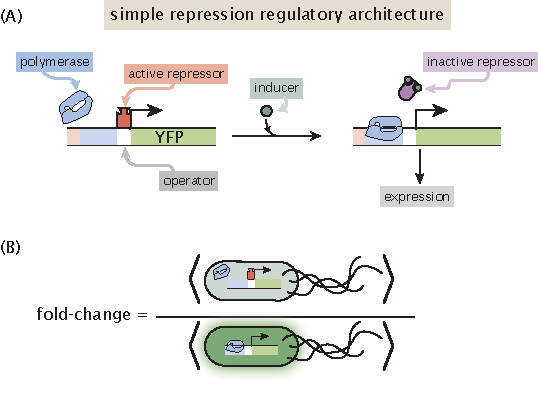
\includegraphics{../figs/fig1}
  \caption{\textbf{The simple repression regulatory architecture.} (A) A repressor
   binds a specific operator site (white rectangle) on the DNA,
  occluding the binding of a polymerase to the promoter (blue rectangle). In
  the presence of an inducer, the inactive state of the repressor is stabilized,
  allowing the polymerase to bind to the promoter and initiate transcription. (B)
  The fold-change in gene expression is defined as the expression of a fluorescent
  protein in a cell containing a given number of repressors $R$ relative to the
  constitutively expressing strain with zero repressors.}
  }\label{fig:simple_repression}
\end{figure}


\begin{figure}[h]
\centering{
  \includegraphics{../figs/fig1_flowchart}
\caption{\textbf{Scheme of the work.} A set of bacterial strains were measured
using flow cytometry and single-cell microscopy. Each method requires a set
of automated processing steps such as gating and image segmentation to generate
reproducible data for parameter estimation.}
}\label{fig:flowchart}
\end{figure}

\section*{Materials & Methods}

\section*{Results}
\begin{figure}[ht]
  \centering{
  \includegraphics{../figs/fig2_parameter_estimation}
  \caption{\textbf{Estimation of the inducer binding constants between methods.}
  (A) The fold-change in gene expression is }}
\end{figure}


\begin{figure}[ht]
  \centering{
  \includegraphics{../figs/fig3_distributions}
  \caption{\textbf{Intensity distributions from flow cytometry and microscopy.}}
  }
\end{figure}

\begin{figure}[ht]
  \centering{
  \includegraphics{../figs/fig4_moment_comparison}
  \caption{\textbf{Comparison of central moments of the intensity distributions.}}
  }
\end{figure}
\end{document}
